% !TeX spellcheck = en_GB
\chapter{Main Objectives}
\section{Overview}
The goal of this project is to design, implement and provide a guidance Platform for development Country, e.g. Afghanistan. Taking the circumstances in such development Country in account, the platform should provide the users of IT-Systems with the knowledge to assure the sustainability of IT-Systems in their countries. Besides providing general information of the IT-Systems, the platform should provide, similar as in the “BSI Grundschutzkatalog”, information aiming to localize and solve problematics that may occur to the IT-Systems as a result of a human error, technical failure or a catastrophe etc. 
\\
\begin{figure}[h]
    \centering
    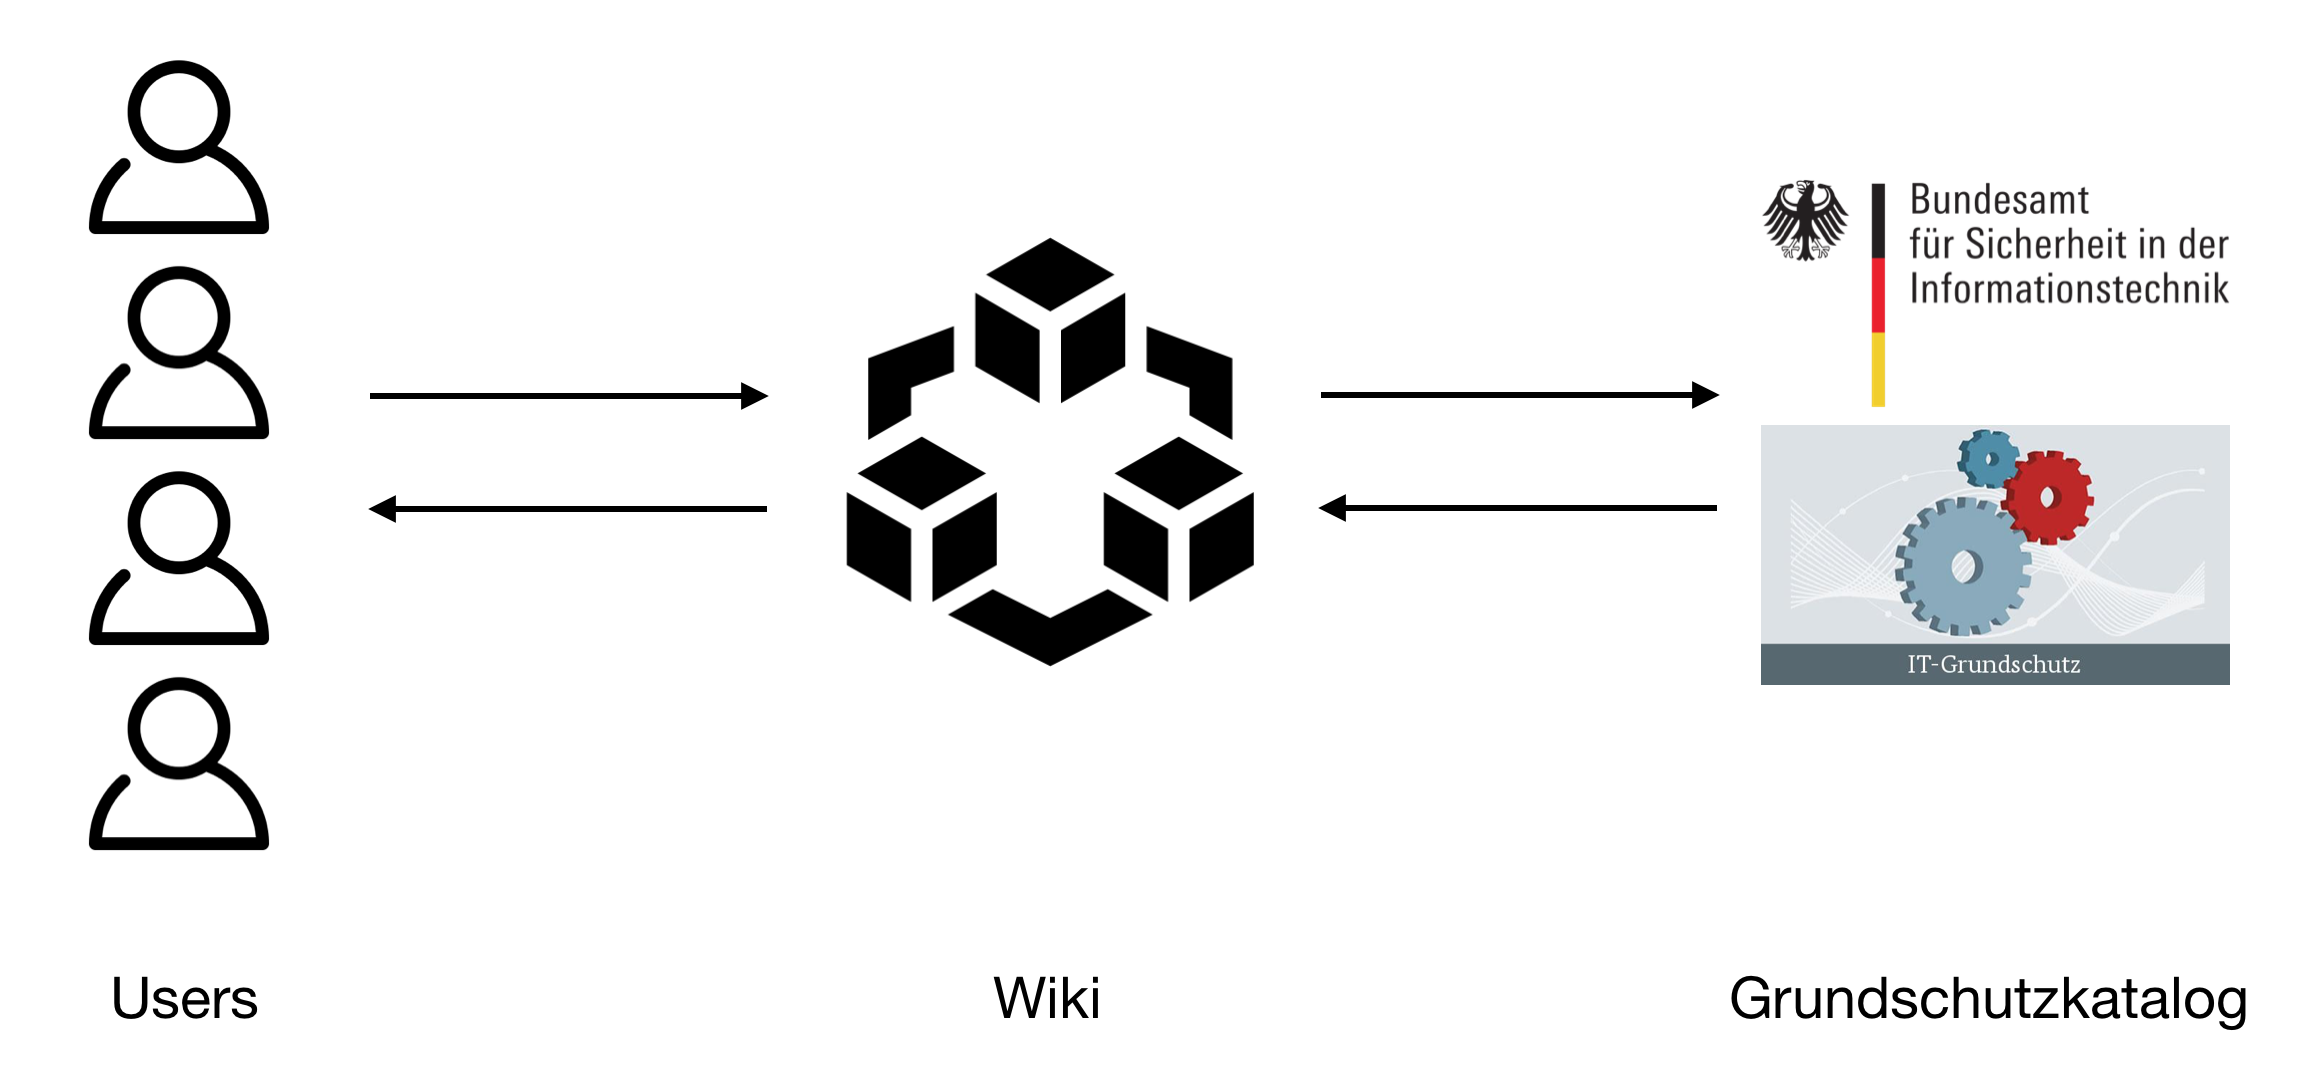
\includegraphics[scale=0.3]{Pictures/ConceptSketch}
    \caption{Abstract System Design}
\end{figure}

\section{Wiki}
Considering the limited availability of IT-specialists in most of the development countries, and after reviewing the possible ways to design and provide the platform, our team considers it convenient to create an open Platform in which people can collaboratively add, edit, delete or archive content, similar to Wikipedia. This should allow the platform to constantly grow and stay relevant to the current circumstances. However, this should not mean that everyone can write whatever content for everybody to read. To assure that, we have to set rules and access permission levels. 

\section{Archive}
\label{archive}
The Website should always be up to date, but we also want to offer the possibility to look up the old content. For this we need an archive,
the archive stores information that is no longer up-to-date but could be still relevant for some user. For example: If users are looking for a problem such as a - no longer supported operating system - and there are no information in the Wiki regarding this problem, he could find older approaches in the archive. 
\section{User types}
In the following section will be discussed the different user roles and their functions. We decided to create 4 types of users with different user rights. This is illustrated in the appendix by the use case diagrams. 
\\
\textbf{Guest}, the guest has the possibility to browse and search in the archive and also in the wiki. The search can be refine with several options (more information about the search in the text search section). If the guest is not sure how to find his problem he can use the Wizard (more information in the Wizard section). In the wiki are news from different topics which the guest can check out.

\textbf{User}, every registered user can write articles in the wiki and change them with the functions: create content and edit content. They also can edit their profile. The content manager can proceed to use all functions of the guest.

\textbf{Moderator} (Mod), will be appointed for a specific topic for example “b2 infrastructure”. The mod is responsible for moderating articles, which means to delete wrong or inappropriate content or make it recognizable for users that the article is unverified. They create the news and they are also responsible - if necessary - to ban content manager. The Mod can proceed to use all functions of the user.

\textbf{Admin}, the admin is responsible for appointing the Mods and remove them if necessary. He also manages the topics, which means creating new topics, removes old ones and controls that each topic got a Mod. For new topics or new mods, the admin sets new permissions or changes them. One of the most important tasks is to update the BSI catalog as soon as a new one is available and to move the old one to the archive. The admin can use all functions of the Mod.
\section{BSI Catalog}
The English version of the BSI catalogue has been published in a single PDF file. This makes browsing, or even searching a specific problem, a difficult task for beginners. Therefore the BSI Catalogue should be added as an "locked" Article, only modifiable by Administrators.
\\\\
In fact, converting catalogues in articles by hand would be an interminable task. Accordingly, a parser is needed. This parser will analyse the PDF file and create the article automatically. Further, the BSI provides cross-reference tables of the catalogue. These amend the useful links inside each subsection and could be used to recommend cross-referenced counter-measures to specific threats.

\section{Text search}
\label{search_function}
A text search function allows users of the platform a possibility to make a free text search request and browse the results containing the key-words. Users should also have the opportunity to narrow their search request by selecting a specific topic in which they would like to find results. These topic are: "All", "News", "Module", "Threats", "Counter-Measures", "Archive". Choices should be available as a dropdown list.
\\\\
The search field should be well placed on the home page. The system should have a function "Back to the search results". The search function should have fault tolerance, as well as ability to deal with synonyms. Fault tolerance means that the user will get the result even if he misspells a word or if he uses singular or plural. While a non-fault-tolerant search will let the visitor go nowhere, the system should nevertheless display the appropriate results.
In addition Search functions, which also master synonyms, do even more. For example, the system should derive results from the search input "laptop" in which the word "notebook" appears and for this purpose access an extensive database of words of the same meaning. The automatic completion of search terms is very welcome.

\section{Wizzard}
\label{wizard}
Beginners who are not familiar with the terminology may have a hard time finding solutions to problems they encounter. To help them, we would like to implement a "Wizzard", which will ask them a set of yes/no questions to filter out what problems they could have, similar to the game Akinator\footnote{\url{http://en.akinator.com}}. 

\section{Frontpage}
The frontpage is the entry point to the different services offered by the website. 
As such its design should provide a clear overview of and a dead on target guidance to all available functions for users of all levels of experience.
Firstly, the frontpage also displays the always present top section (see section~\ref{top_section}) but no side bar.
Directly below the top section is a distinguished area for time-critical news which inform of widespread threats or important updates.
In times of no imminent danger time-critical news might not be displayed but instead a few of the most recent regular news which are part of the wiki.
The third area in a vertical sense is a wide and inviting search bar that allows experienced users the quick access to the BSI catalogue and other parts. 
The search offers the full functionality as described in section~\ref{search_function}.
As a last section before the always present bottom section is an overview of introductory tutorials on how to implement the guidelines of the BSI \todo{typo}catalgue while developing, building and maintaining a basic IT system.
Equally visible as the tutorials should be the offer to use the wizard to help and find security gaps and other system flaws.
Both the tutorials and the wizard are aimed at users of no or little knowledge or overview of the BSI catalogue.
For detailed explanations see section~\ref{tutorials} for the tutorials and section~\ref{wizard} for the wizard.
\todo[inline]{would be nice to have a sketch to illustrate all this}
 
\section{Top Section}
\label{top_section}

The top section is an always present area at the top of each subpage that connects the different services and allows for quick access.
It should feature the following items whose order and wording might be changed appropriately:
\begin{itemize}
    \item Home/Frontpage
    \item News
    \item Browse the BSI catalogue/Wiki (????)
    \item Tutorials
    \item Wizard
    \item Search
    \item Login 
        .
\end{itemize}
\todo[inline]{same as Frontpage, an illustrating sketch would make it nicer}
\section{Tutorials}
\label{tutorials}

Tutorials should call unexperienced users' attention to the most important points in the BSI catalogue when developing, building or maintaining an IT infrastructure.
They could briefly explain mayor points of the BSI catalogue and indicate next steps.
The simplest tutorial could simply introduce the usage and goal of the website and its subservices.
The tutorials are not meant to be a rewrite - i.e. the BSI catalogue for dummies - but thought of as a quick overview and guiding introduction into the matter.
They are part of the wiki and as such created and maintained by content manager and linked by mods.
\todo[inline]{to remove?}
